
\chapter{Figure of the Earth}

\begin{figure}[ht]
    \vspace{-45pt}
    %\begin{adjustwidth}{-1cm}{-0cm}
        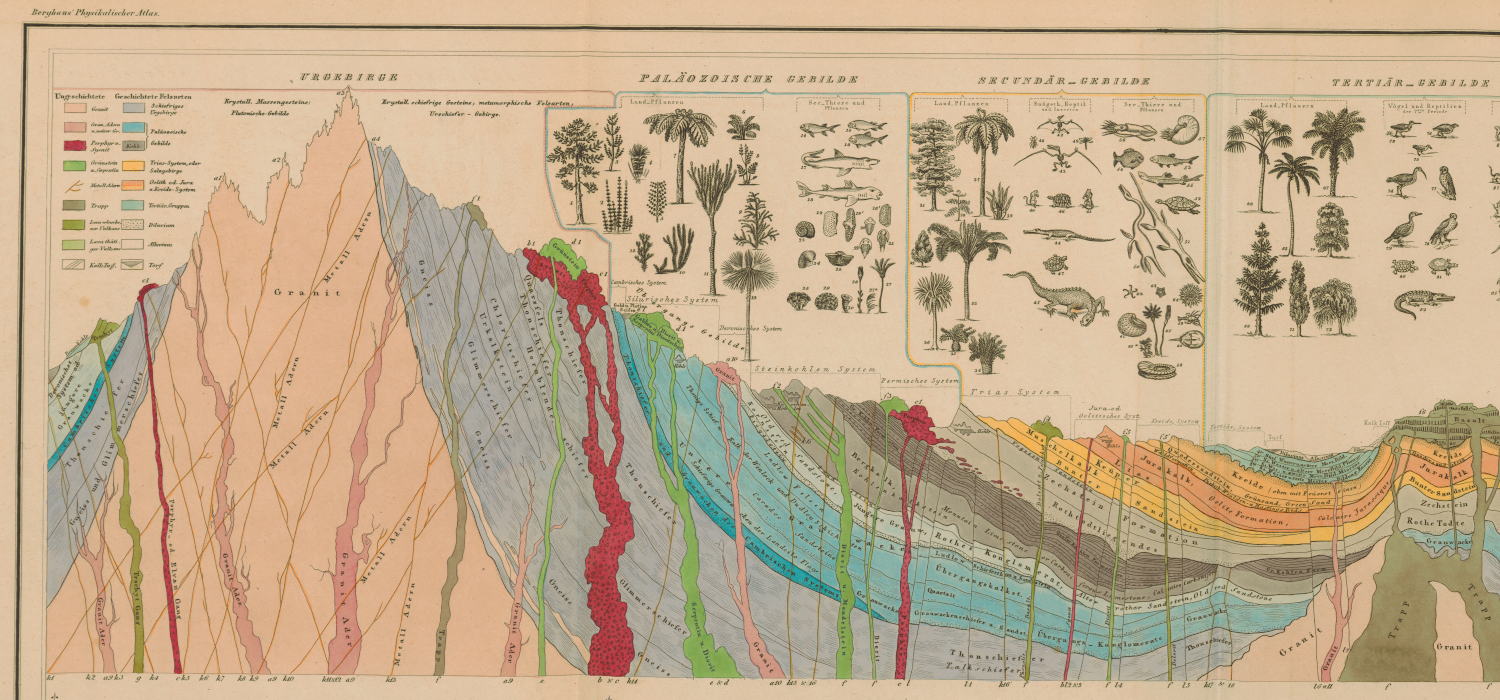
\includegraphics[width=\linewidth]{../../pictures/Alexander_von_Humboldt_-_1841_-_Diagram_of_a_cross-section_of_the_earth's_crust-small-2.png}
        \captionsetup{width = \linewidth}
        \caption{\footnotesize Alexander von Humboldt, diagram of a cross-section of the earth's crust, 1841. Public domain.}
    %\end{adjustwidth}
\end{figure}
\clearpage

\lettrine[lines = 4]{\goudy T}{he} delineation of the principal characteristics of telluric phenomena must begin with the form of our planet and its relations in space. Here, too, we may say that it is not only the mineralogical character of rocks, whether they are crystalline, granular, or densely fossiliferous, but the geometrical form of the Earth itself, which indicates the mode of its origin, and is, in fact, its history. An elliptical spheroid of revolution gives evidence of having once been a soft or fluid mass. Thus, the Earth's compression constitutes one of the most ancient geognostic events, as every attentive reader of the book of nature can easily discern; and an analogous fact is presented in the case of the Moon, the perpetual direction of whose axes toward the Earth, that is to say, the increased accumulation of matter on that half of the Moon which is turned toward us, determines the relations of the periods of rotation and revolution, and is probably cotemporaneous with the earliest epoch in the formative history of this satellite. The mathematical figure of the Earth is that which it would have were its surface covered entirely by water in a state of rest; and it is this assumed form to which all geodesical measurements of degrees refer. This mathematical surface is different from that true physical surface which is affected by all the accidents and inequalities of the solid parts.\footnote{Bessel, Aligemeine Betrachtungen aber Gradmessungen nach astronomischgeodatischen Arbeiten, at the conclusion of Bessel and Baeyer, Gradmessung in Ostpreussen, 8. 427. Regarding the accumulation of matter on the side of the Moon turned toward us (a subject noticed in an earlier part of the text), see Laplace, Expos. du Syst. du Monde,p. 308.} The whole figure of the Earth is determined when we know the amount of the compression at the poles and the equatorial diameter; in order, however, to obtain a perfect representation of its form, it is necessary to have measurements in two directions, perpendicular to one another.

Eleven measurements of degrees (or determinations of the curvature of the Earth's surface in different parts), of which nine only belong to the present century, have made us acquainted with the size of our globe, which Pliny named a point in the immeasurable universe.\footnote{Plin., ii., 68. Seneca, Nat. Quest., Pref.,c. ii. El mundo es poco (the Earth is small and narrow), writes Columbus from Jamaica to Queen Isabella on the 7th of July, 1503; not because he entertained the philosophic views of the aforesaid Romans, but because it appeared advantageous to him to maintain that the journey from Spain was not long, if, as he observes, we seek the east from the west. Compare my Examen Crit. de V Hist. de la G\'{e}ogr. du lime Si\'{e}cle, t.i., p. 83, and t. il., p. 327, where I have shown that the opinion maintained by Delisle, Fr\'{e}ret, and Gosselin, that the excessive differences in the statements regarding the Earth's circumference, found in the writings of the Greeks, are only apparent, and dependent on different values being attached to the stadia, was put forward as early as 1495 by Jaime. Ferrer, in a proposition regarding the determination of the line of demarkation of the papal dominions.} If these measurements do not always accord in the curvatures of different meridians under the same degree of latitude, this very circumstance speaks in favor of the exactness of the instruments and the methods employed, and of the accuracy and the fidelity to nature of these partial results. The conclusion to be drawn from the increase of forces of attraction (in the direction from the equator to the poles) with respect to the figure of a planet is dependent on the distribution of density in its interior. Newton, from theoretical principles, and perhaps likewise prompted by Cassini's discovery, previously to 1666, of the compression of Jupiter,\footnote{Brewster, Life of Sir Isaac Newton, 1831, p. 162. The discovery of the spheroidal form of Jupiter by Cassini had probably directed the attention of Newton to the determination of its cause, and, consequently, to the investigation of the true figure of the Earth. Although Cassini did not announce the amount of the compression of Jupiter (,,th) . till 1691 (Anciens M\'{e}moires de V Acad. des Sciences, t. ti., p. 108), yet we know from Lalande (Astron., 3me \'{e}d., t. iii., p. 335) that Moraldi possessed some printed sheets of a Latin work, On the Spots of the Planets, commenced by Cassini, from which it was obvious that he was aware of the compression of Jupiter before the year 1666, and therefore at least twenty-one years before the publication of Newton's Principia.} determined,

in his immortal work, Philosophie Naturalis Principia, that the compression of the Earth, as a homogeneous mass, was g1,th. Actual measurements, made by the aid of new and more perfect analysis, have, however, shown that the compression of the poles of the terrestrial spheroid, when the density of the strata is regarded as increasing toward the center, is very nearly $\frac{1}{300}$th.

\clearpage
\begin{wrapfigure}{r}{.4\textwidth}
    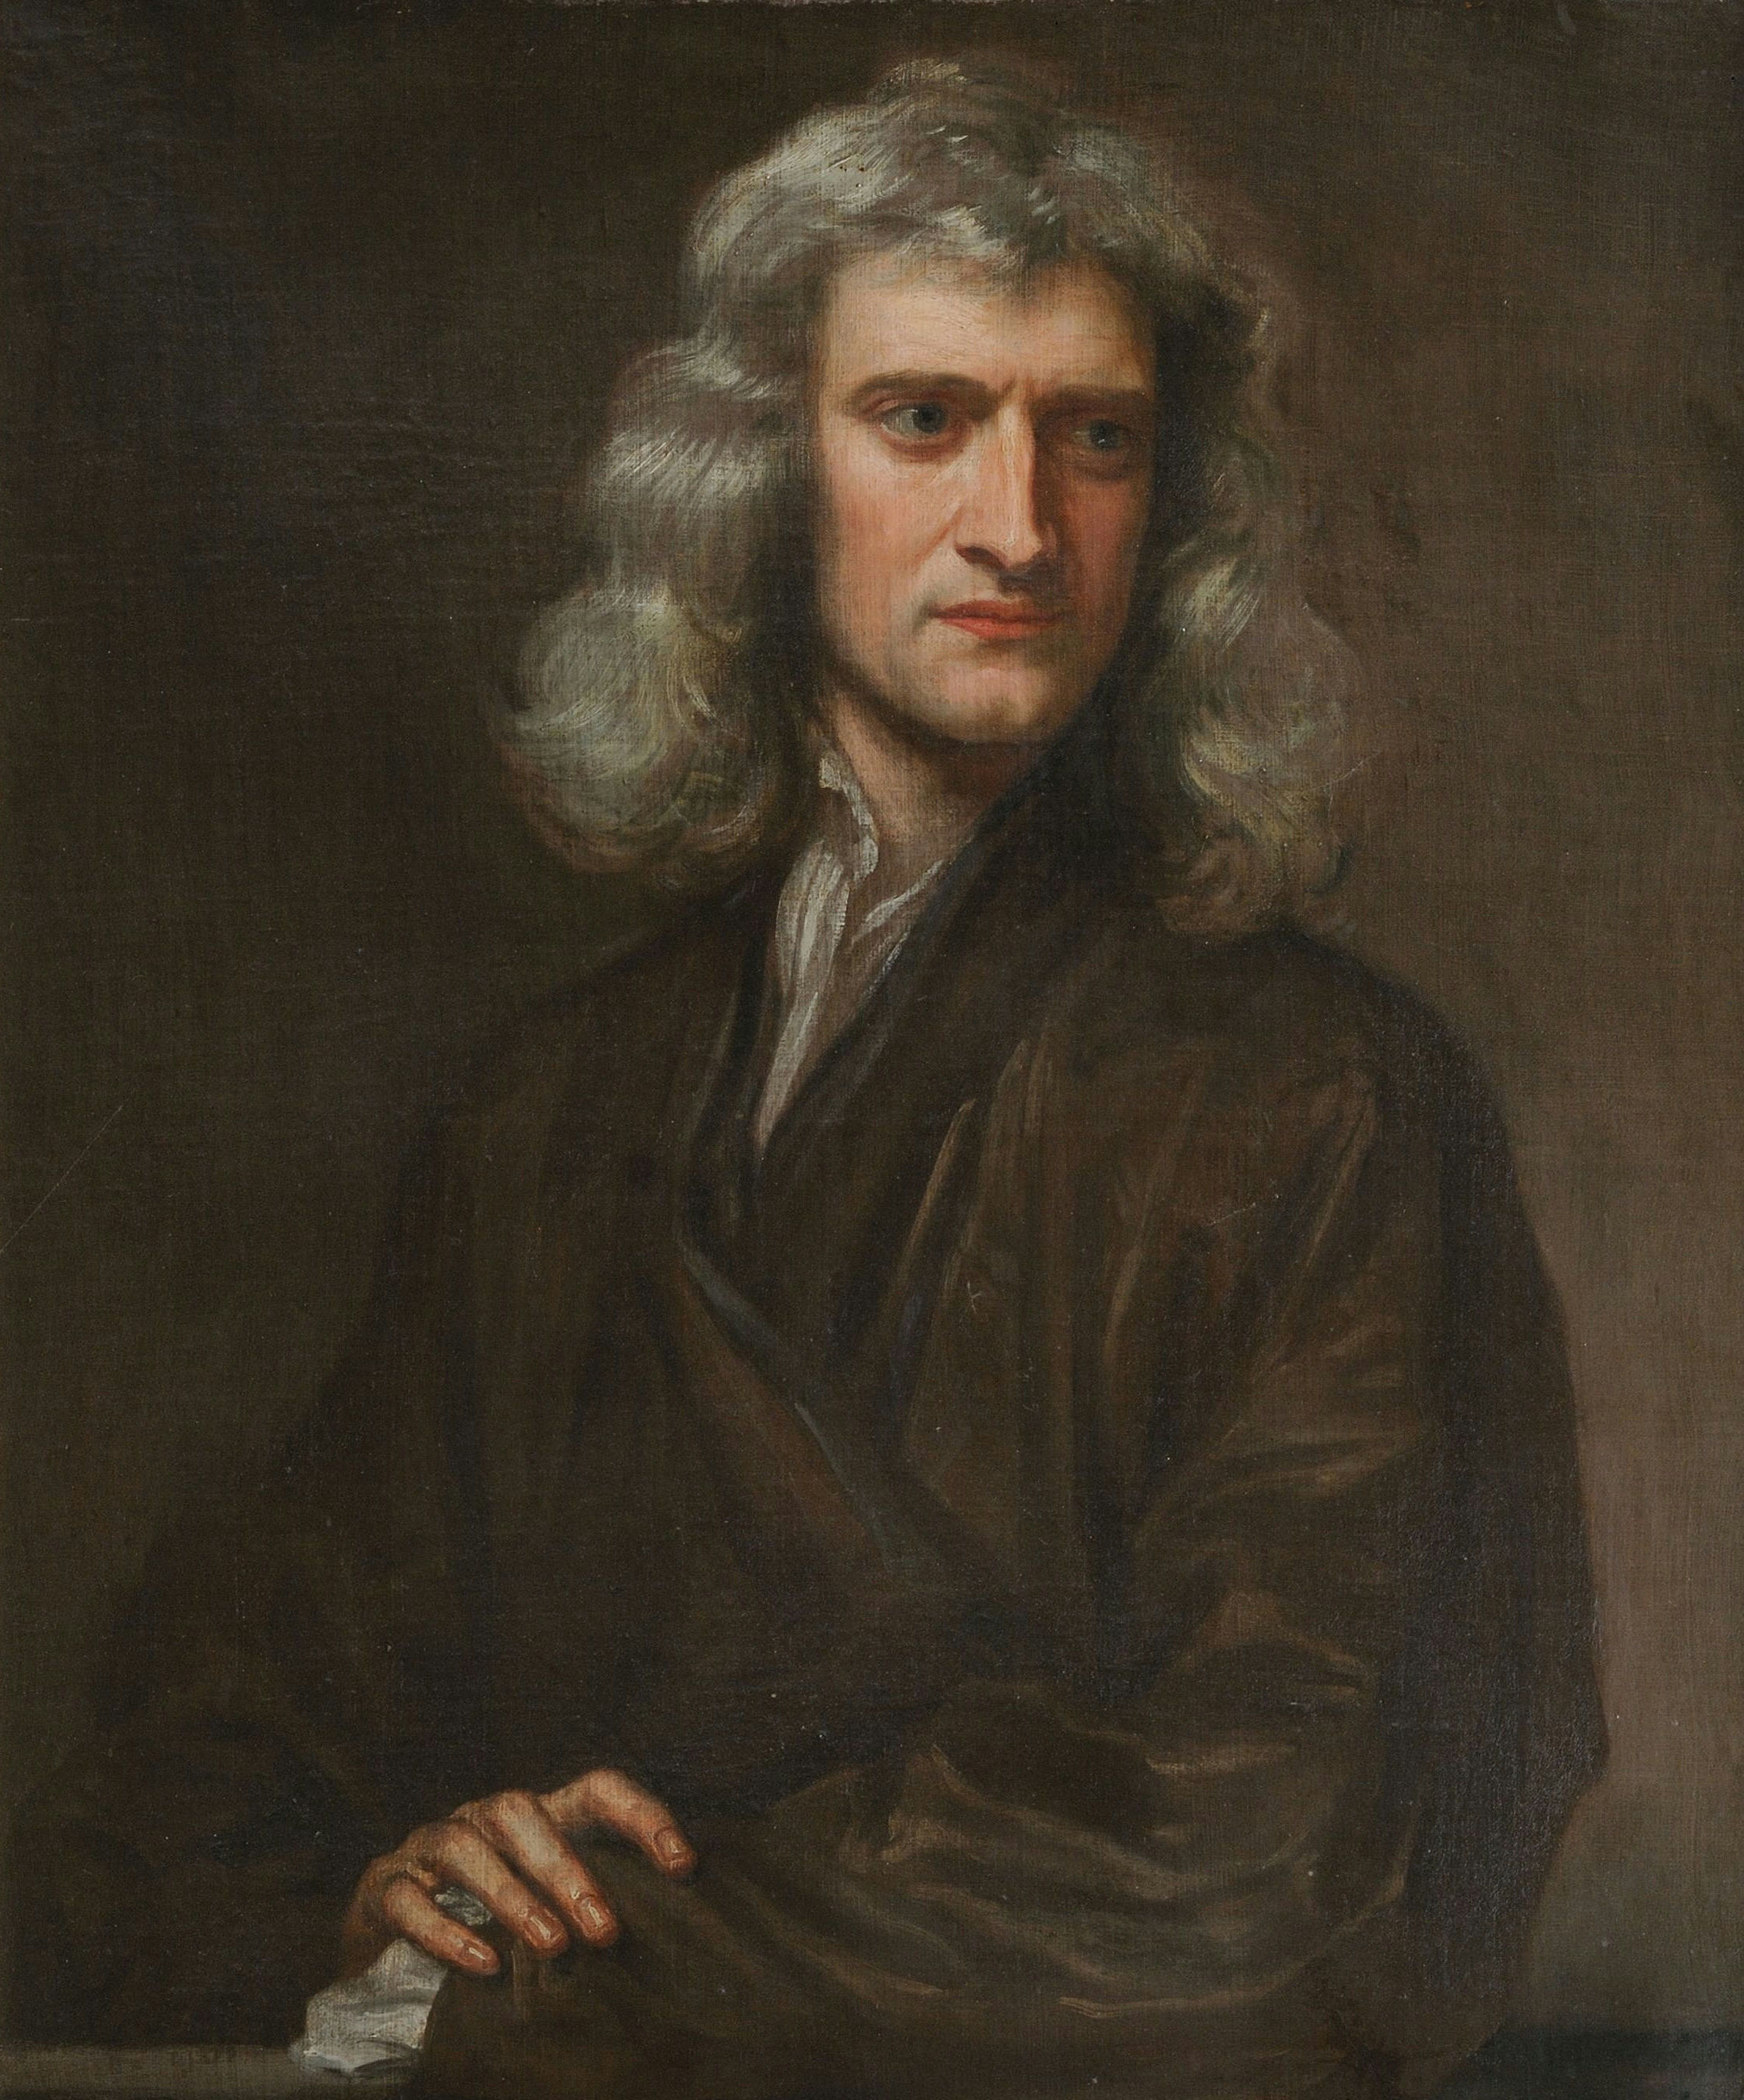
\includegraphics[width=.4\textwidth]{../../pictures/Portrait_of_Sir_Isaac_Newton,_1689.jpg}
    \caption{\footnotesize Sir Isaac Newton (25 December 1642 -- 20 March 1726/27) was a key figure in the philosophical revolution known as the Enlightenment. His book \emph{Philosophiae Naturalis Principia Mathematica} (1687) established classical mechanics. (Source: \href{https://en.wikipedia.org/wiki/Isaac_Newton}{Wikipedia}). Painting of Newton by Godfrey Kneller is in the public domain.}
    \vspace{-.5cm}
 \end{wrapfigure}

Three methods have been employed to investigate the curvature of the Earth's surface, viz., measurements of degrees, oscillations of the pendulum, and observations of the inequalities in the Moon's orbit. The first is a direct geometrical and astronomical method, while in the other two we determine from accurately observed movements the amount of the forces which occasion those movements, and from these forces we arrive at the cause from whence they have originated, viz., the compression of our terrestrial spheroid. In this part of my delineation of nature, contrary to my usual practice, I have instanced methods because their accuracy affords a striking illustration of the intimate connection existing among the forms and forces of natural phenomena, and also because their application has given occasion to improvements in the exactness of instruments (as those employed in the measurements of space) in optical and chronological observations; to greater perfection in the fundamental branches of astronomy and mechanics in respect to lunar motion and to the resistance experienced by the oscillations of the pendulum; and to the discovery of new and hitherto untrodden paths of analysis. With the exception of the investigations of the parallax of stars, which led to the discovery of aberration and nutation, the history of science presents no problem in which the object attained—the knowledge of the compression and of the irregular form of our planet—is so far exceeded in importance by the incidental gain which has accrued, through a long and weary course of investigation, in the general furtherance and improvement of the mathematical and astronomical sciences. The comparison of eleven measurements of degrees (in which are included three extra-European, namely, the old Peruvian and two East Indian) gives, according to the most strictly theoretical requirements allowed for by Bessel,\footnote{According to Bessel's examination of ten measurements of degrees, in which the error discovered by Puissant in the calculation of the French measurements is taken into consideration (Schumacher, Astron. Nachr., 1841, No. 438, s. 116), the semiaxis major of the elliptical naman of revolution to which the irregular figure of the Earth most closely approximates is 3,272,07714 toises, or 20,924,774 feet; the semiaxis minor, 3,261,15983 toises, or 20,854,821 feet; and the amount of compression or eccentricity 555;254; the length of a mean degree of the meridian, 57 013109 toises, or 364,596 feet, with an error of 28403 toises, or 1816 feet, whence the length of a geographical mile is 380723 toises, or 60867 feet. Previous combinations of measurements of degrees varied between ,i,d and 544th; thus Walbeck (De Forma et Magnitudine telluris in demensis arcubus Meridiani definiendis, 1819) gives y57gth Ed. Schmidt (Lehrbuch der Mathem. und Phys. Geographie, 1829, s. 5) gives gyz54, as the mean of seven measures. Respecting the influence of great differences of longitude on the polar compression, see Bibliotheque Universelle, t. xxxiii., p. 181, and t. xxxv., p. 56; likewise Connaissance des Tems, 1829, p.290. From the Itmarinequalities alone, Laplace (Exposition du Syst. du Monde, p.229) found it, by the older tables of Burg, to be gerzth; and subsequently, from the lunar observations of Burckhardt and Bouvard, he fixed it at zoyyth (M\'{e}canique C\'{e}leste, t. v., p. 13 and 43).} a compression of $\frac{1}{299}$th. In accordance with this, the polar radius is 10,938 toises (69,944 feet), or about $11\frac{1}{2}$ miles, shorter than the equatorial radius of our terrestrial spheroid. The excess at the equator in consequence of the curvature of the upper surface of the globe amounts, consequently, in the direction of gravitation, to somewhat more than 43th times the height of Mont Blanc, or only 2 times the probable height of the summit of the Dhawalagiri, in the Himalaya chain. The lunar inequalities (perturbation in the Moon's latitude and longitude) give, according to the last investigations of Laplace, almost the same result for the ellipticity as the measurements of degrees, viz., z,th. The results yielded by the oscillation of the pendulum give, on the whole, a much greater amount of compression, viz., $\frac{1}{288}$th.\footnote{The oscillations of the pendulum give z3'g.zth as the g\'{e}neral result of Sabine's great expedition (1822 and 1823, from the equator to 80 north latitude); according to Freycinet, 5,15, exclusive of the experiments instituted at the Isle of France, Guam, and Mowi (Mawi); according to Forster, 5,5.5th; according to Duperrey, 5,4,,th; and according to Liitke (Partie Nautique, 1836, p. 232), giyth, calculated from eleven stations. On the other hand, Mathieu (Connaiss. des. 'emps, 1816, p. 330) fixed the amount at .,1,,d, from observations made between Formentera and Dunkirk; and Biot, at ,1,th, from observations between Formentera and the island of Unst. Compare Baily, Report on Pendulum Experiments, in the Memoirs of the Royal Astronomical Society, vol. vii., p. 96; also Borenius, in the Bulletin de l'Acad. de St. P\'{e}tersbourg, 1843, t.i., p.25. The first proposal to apply the length of the pendulum as a standard of measure, and to establish the third part of the seconds pendulum (then supposed to be every where of equal length) as a pes horarius, or Baegeal waeseufo) that might be recovered at any age and by all nations, is to be found in Huygens's Horologium Oscillatorium, 1673, Prop. 25. A similar wish was afterward publicly expressed, in 1742, on a monument erected at the equator by Bouguer, La Condamine, and Godin. On the beautiful marble tablet which exists, as yet uninjured, in the old Jesuits' College at Quito, I have myself read the inscription, Penduli simplicis equinoctialis untus minuti secundi archetypus, mensure naturalis exemplar, utinam universalis From an observation made by La Condamine, in his Journal du Voyage al Equateur, 1751, p. 163, regarding parts of the inscription that were not filled up, and a slight difference between Bouguer and himself respecting the numbeys, I was led to expect that I should find considerable discrepancies between the marble tablet and the inscription as it had been described in Paris; but, after a careful comparison, I merely found two perfectly unimportant differences ex arcu graduum 34 instead of ex arcu graduum plusquam trium, and the date of 1745 instead of 1742. The latter circumstance is singular, because La Condamine returned to Europe in November, 1744, Bouguer in June of the same year, and Godin had left South America in July, 1744. The most necessary and useful amendment to the numbers on this inscription would have been the astronomical longitude of Quito. (Humboldt, Recueil d'Odserv. Astron., t. ii., bp. 319354.) Nouet's latitudes, engraved on Egyptian monuments, offer a more recent example of the danger presented by the grave perpetuation of false or careless results.}


Galileo, who first observed when a boy (having, probably, suffered his thoughts to wander from the service) that the height of the vaulted roof of a church might be measured by the time of the vibration of the chandeliers suspended at different altitudes, could hardly have anticipated that the pendulum would one day be carried from pole to pole, in order to determine the form of the Earth, or, rather, that the unequal density of the strata of the Earth affects the length of the seconds pendulum by means of intricate forces of local attraction, which are, however, almost regular in large tracts of land. These geognostic relations of an instrument intended for the measurement of time, this property of the pendulum, by which, like a sounding line, it searches unknown depths, and reveals in volcanic islands,\footnote{Respecting the augmented intensity of the attraction of gravitation in volcanic islands (St. Helena, Ualan, Fernando de Noronha, Isle of France, Guam, Mowi, and Galapagos), Rawak (Liitke, p. 240) being an exception, probably in consequence of its proximity to the highland of New Guinea, see Mathieu, in Delambre, Hist. de 1 Astronomie, au 18me Siècle, p. 701.} or in the declivity of elevated continental mountain chains,\footnote{Numerous observations also show great irregularities in the length of the pendulum in the midst of continents, and which are ascribed to local attractions. (Delambre, Mesure de la Méridienne, t. iii., p. 548; Biot, in the Mém de Académie des Sciences, t. viii., 1829, p. 18 and 23.) In passing over the South of France and Lombardy from west to east, we find the minimum intensity of gravitation at Bordeaux; from thence it increases rapidly as we advance eastward, through Figeac, Clermont-Ferrand, Milan, and Padua; and in the last town we find that the intensity has attained its maximum. The influence of the southern declivities of the Alps is not merely dependent on the general size of their mass, but (much more), in the opinion of Elie de Beaumont (Rech. sur les Révol. de la Surface du Globe, 1830, p. 729), on the rocks of melaphyre and serpentine, which have elevated the chain. On the declivity of Ararat, which with Caucasus may be said to lie in the center of gravity of the old continent formed by Europe, Asia, and Africa, the very exact pendulum experiments of Fedorow give indications, not of subterranean cavities, but of dense volcanic masses. (Parrot, Reise zum Ararat, bd. ii., s. 143.) In the geodesic operations of Carlini and Plana, in Lombardy, differences ranging from 20 to 478 have been found between direct observations of latitude and the results of these operations. (See the instances of Andrate and Mondovi, and those of Milan and Padua, in the Opérations Geodes. et Astron. pour la Mesure d'un Arc du Parallèle Moyen, t. ii., p. 347; Effemeridi Astron. di Milano, 1842, p. 57.) The latitude of Milan, deduced from that of Berne, according to the French triangulation, is 45 27 52, while, according to direct astronomical observations, it is 45 27 35. As the perturbations extend in the plain of Lombardy to Parma, which is far south of the Po (Plana, Opérat. Geod., t. ii., p. 847), it is probable that there are deflecting causes concealed beneath the soil of the plain itself. Struve has made similar experiments with corresponding results in the most level parts of eastern Europe. (Schumacher, Astron. Nachrichten, 1830, No. 164, s. 399.) Regarding the influence of dense masses supposed to lie at a small depth, equal to the mean height of the Alps, see the analytical expressions given by Hossard and Rozet, in the Comptes Rendus, t. xviii., 1844, p. 292, and compare them with Poisson, Traité de Mécanique (2me éd.), t. i., p. 482. The earliest observations on the influence which different kinds of rocks exercise on the vibration of the pendulum are those of Thomas Young, in the Philos. Transactions for 1819, p. 7096. In drawing conclusions regarding the Earth's curvature from the length of the pendulum, we ought not to overlook the possibility that its crust may have undergone a process of hardening previously to metallic and dense basaltic masses having penetrated from great depths, through open clefts, and approached near the surface.} dense masses of basalt and melaphyre instead of cavities, render it difficult, notwithstanding the admirable simplicity of the method, to arrive at any great result regarding the figure of the Earth from observation of the oscillations of the pendulum. In the astronomical part of the determination of degrees of latitude, mountain chains, or the denser strata of the Earth, likewise exercise, although in a less degree, an unfavorable influence on the measurement. As the form of the Earth exerts a powerful influence on the motions of other cosmical bodies, and especially on that of its own neighboring satellite, a more perfect knowledge of the motion of the latter will enable us reciprocally to draw an inference regarding the figure of the Earth. Thus, as Laplace ably remarks,\footnote{Laplace, Expos. du Syst. du Monde, p. 231.} An astronomer, without leaving his observatory, may, by a comparison of lunar theory with true observations, not only be enabled to determine the form and size of the Earth, but also its distance from the Sun and Moon results that otherwise could only be arrived at by long and arduous expeditions to the most remote parts of both hemispheres.

The compression which may be inferred from lunar inequalities affords an advantage not yielded by individual measurements of degrees or experiments with the pendulum, since it gives a mean amount which is referable to the whole planet. The comparison of the Earth's compression with the velocity of rotation shows further the increase of density from the strata from the surface toward the center, an increase which a comparison of the ratios of the axes of Jupiter and Saturn with their times of rotation likewise shows to exist in these two large planets. Thus, the knowledge of the external form of planetary bodies leads us to draw conclusions regarding their internal character.

The northern and southern hemispheres appear to present nearly the same curvature under equal degrees of latitude, but,as has already been observed, pendulum experiments andmeasurements of degrees yield such different results for individual portions of the Earths surface that no regular figureean be given which would reconcile all the results hithertoobtained by this method. The true figure of the Earth is toa regular figure as the uneven surfaces of water in motion areto the even surface of water at rest.